\documentclass[11pt]{article}
\usepackage[margin=1in]{geometry}
\usepackage[utf8]{inputenc}
\usepackage[english]{babel}

\usepackage{pslatex}

\usepackage[pdftex]{graphicx}
\usepackage{siunitx}
\usepackage{caption}

\usepackage{booktabs,array}
\usepackage{tikz}
\usetikzlibrary{matrix,calc}
\usetikzlibrary{decorations.pathreplacing,angles,quotes}
\usetikzlibrary{bayesnet}
\usetikzlibrary{shapes.geometric,fit}

\newlength{\tikzheight}
\newlength{\tikzwidth}

\usepackage{amsfonts,amsmath,amssymb}
\usepackage{mathtools}
\usepackage{multicol}
\usepackage{multirow}
\usepackage{xcolor}
\usepackage{multicol}
\usepackage{algorithm}
\usepackage{algpseudocode}
\usepackage{adjustbox,lipsum}

\usepackage[hidelinks,breaklinks]{hyperref}

\usepackage{minted}
\usemintedstyle{emacs}

\definecolor{c1}{RGB}{39,64,139}
\definecolor{c2}{RGB}{30,144,255}
\definecolor{c3}{RGB}{255,165,0}
\definecolor{c4}{RGB}{205,205,0}
\definecolor{c5}{RGB}{139,139,0}

\newcommand{\secref}[1]{\S\,\ref{#1}}
\newcommand{\appref}[1]{Appendix~\ref{#1}}
\newcommand{\figref}[1]{Fig.~\ref{#1}}
\newcommand{\tabref}[1]{Tab.~\ref{#1}}

\newcommand{\abs}[1]{\ensuremath\left|#1\right|}

\newcommand{\ie}{\emph{i.e.}}
\newcommand{\eg}{\emph{e.g.}}
\newcommand{\etc}{\emph{etc.}}

%
% The following macro is used to generate the header.
%
\newcommand{\lecture}[4]{
   \pagestyle{myheadings}
   \thispagestyle{plain}
   \noindent
   \begin{center}
   \framebox{
      \vbox{\vspace{1mm}
    \hbox to 6.58in {Technology and AI Learning Seminar (TAILS) \hfill Montana State University} 
    \hbox to 6.58in {Spring 2023 \hfill Dept. of Mathematics Sciences}
       \vspace{4mm}
       \hbox to 6.28in {\large\bf\hfill Lecture #1: #2  \hfill}
       \vspace{4mm}
       \hbox to 6.28in {\footnotesize Lecturer: #3 \hfill Scribe: #4}
      \vspace{1mm}}
   }
   \end{center}
   \markboth{Lecture #1: #2}{Lecture #1: #2}
   \vspace*{4mm}
}

\renewcommand{\vec}[1]{\ensuremath\mathbf{#1}}

\begin{document}

%%%%%%%%%%%%%%%%%%%%%%%%%%%%%%%%%%%%%%%%%%%%%%%%%%%%%%%%%%%%%%%%%%%%%%%%%%%%%%%%%%%%%%%%%%%%%%%%%%%%%%%%%%%% FILL IN THE RIGHT INFO.
% \lecture{**LECTURE-NUMBER**}{**DATE**}{**LECTURER**}{**SCRIBE**}
\lecture{1}{Sampling and Quantization}{Dominique Zosso, 2023-02-03}{Trevor Vannoy}
\tableofcontents
\null\hrule
% stay between these lines

\section{Hierarchy of data acquisition and processing}

\begin{figure}
    \centering
    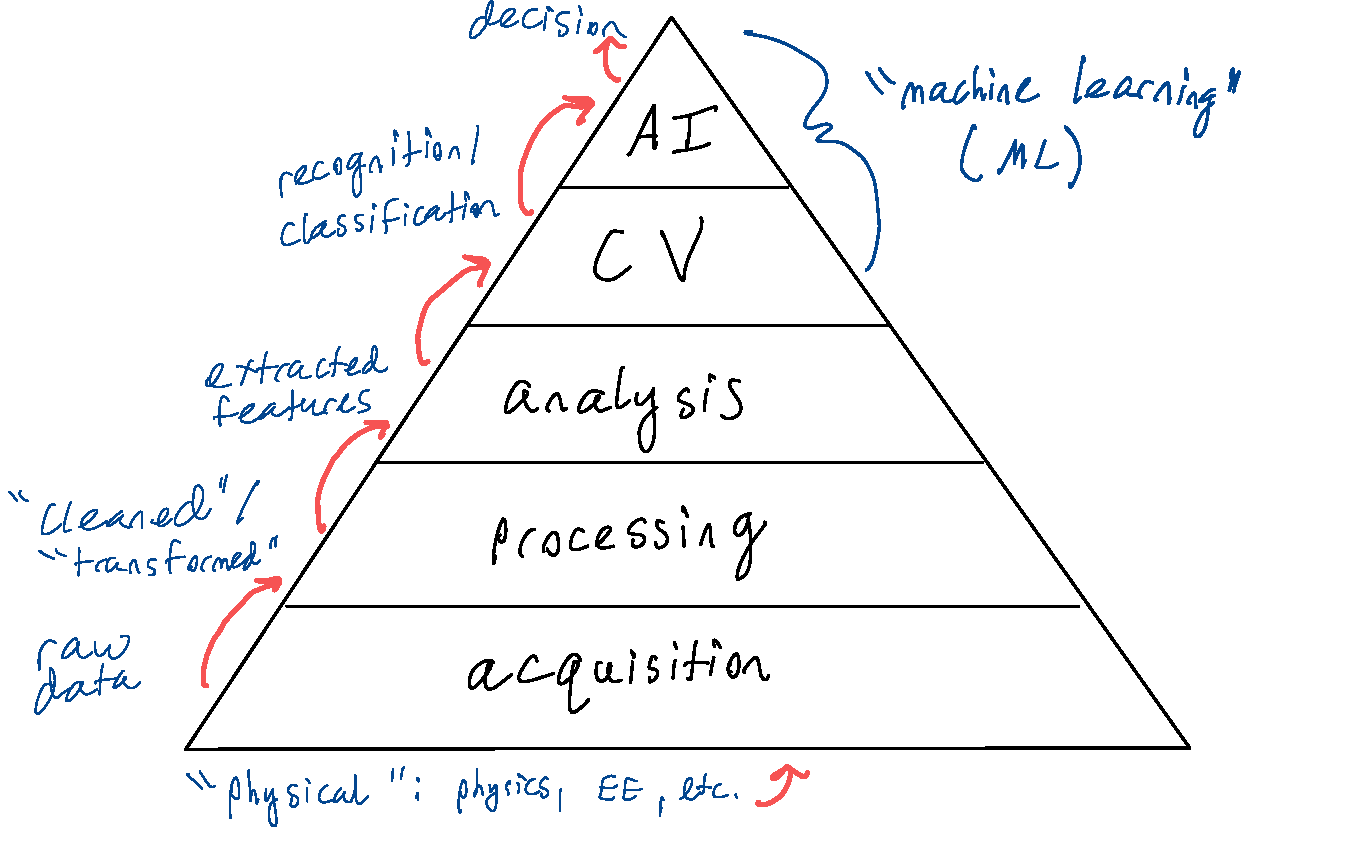
\includegraphics[width=\textwidth]{../figures/lecture01/data-processing-pyramid.pdf}
    \caption{An example of data acquisition and processing steps illustrated as a pyramid.}
    \label{fig:data processing hierarchy}
\end{figure}

Broadly speaking, in ``Data Science'' and related fields (Machine Learning, Artificial Intelligence, Signal Processing, etc.), there is typically a hierarchy of data acquisition and data processing. \figref{fig:data processing hierarchy} shows a nominally-opinionated example of this hierarchy as a pyramid.

At the bottom, we have data acquisition. This is where our raw data comes from. From a traditional signal processing point of view, data acquisition is a ``physical'' process: using sensors to convert ``physical'' parameters into electrical signal (\eg, taking photographs, recording sounds with microphones, measuring light, measuring the flow of fluids, recording location using GPS, recording voltages with an analog-to-digital converter, \etc). Once the data is acquired, the rest of the pyramid is responsible for processing and extracting useful, actionable information out of the raw data. In a broader context, the raw data may also be synthetically generated on a computer, or it might be gathered by some other means (\eg, surveys, censuses, Netflix user movie ratings, eCommerce shopping trends, connections on a social network, \etc). Regardless of how the data is acquired or what the data looks like (e.g., a list of numbers, graphs\footnote{\href{https://en.wikipedia.org/wiki/Graph\_(discrete\_mathematics)}{https://en.wikipedia.org/wiki/Graph\_(discrete\_mathematics)}}), the rest of the pyramid remains the same. Since the topic of this lecture is ``sampling and quantization'' and this seminar is about ``AI in dynamical systems (time series)'', we will focus on ``physical'' acquisition of time series data; however, it is worth keeping the many other types of data in mind.

After data acquisition, we have low-level data processing tasks, such as ``cleaning'' the data (\eg, removing outliers) and/or transforming the data into some more useful format. After the low-level processing, we move onto ``analysis'', which includes extracting features from the data.\footnote{\href{https://en.wikipedia.org/wiki/Feature_extraction}{https://en.wikipedia.org/wiki/Feature\_extraction}}. The next higher level after that is labeled as ``Computer Vision / CV'' in \figref{fig:data processing hierarchy}; although CV is specific to image/video analysis, generally speaking, this step involves pattern recognition/classification and/or regression. Finally, at the top of the pyramid, we have decisions and control actions.

Since the bottom of a pyramid is always the foundation \texttt{:)}, we'll start with the traditional data acquisition processes: sampling and quantization.

\section{Intro to Sampling and Quantization of Time Series}

Since we are primarily interested in time series\footnote{\href{https://en.wikipedia.org/wiki/Time_series}{https://en.wikipedia.org/wiki/Time\_series}}, we need to get some definitions out of the way before diving into sampling and quantization.

The simplest time series is defined as a function $f: \mathbb{R} \rightarrow \mathbb{R}$ that is indexed by time, typically written as $f(t)$. We can also define various other types of time series:
\begin{itemize}
    \item multivariate time series: $\vec{f}: \mathbb{R} \rightarrow \mathbb{R}^m \quad \longrightarrow \quad \begin{bmatrix}f_1(t) & f_2(t) & \hdots & f_m(t)\end{bmatrix}^\top$
    \item multidimensional signals: $f: \mathbb{R}^n \rightarrow \mathbb{R} \quad \longrightarrow \quad f(x,y)$
    \item ``all of the above'': $\vec{f} : \mathbb{R}^n \rightarrow \mathbb{R}^m$, \eg, an RBG image
\end{itemize}

The above definitions are all \emph{continuous} functions/signals. In the abstract, this is fine; however, when using computers, we have to discretize the \emph{domain} (\eg, time, space) and the \emph{co-domain} (\eg, features). Discretizing the \emph{domain} is referred to as \emph{sampling}\footnote{\href{https://en.wikipedia.org/wiki/Sampling_(signal_processing)}{https://en.wikipedia.org/wiki/Sampling\_(signal\_processing)}}, and discretizing the \emph{co-domain} is referred to as \emph{quantization}\footnote{\href{https://en.wikipedia.org/wiki/Quantization_(signal_processing)}{https://en.wikipedia.org/wiki/Quantization\_(signal\_processing)}}. Sampling the is the process of converting a continuous domain into a discrete, (generally) evenly-spaced set of samples (\eg, think of a grid of pixels). Quantization is the process of converting a continuous feature/parameter into a finite number of levels (\eg, a pixel can only take on a finite number of values). Sampling and quantization both result in a loss of information!

For a sampled signal, the index variables are finite and discrete. We'll use the following notation for a one-dimensional time series:
\begin{equation}
    f[k] \;\; k \in \mathbb{Z};
    \label{eq:discrete notation 1d}
\end{equation}
or for a 2-dimensional signal (\eg, an image):
\begin{equation}
    f[i,j] \;\; i,j \in \mathbb{Z}.
    \label{eq:discrete notation 2d}
\end{equation}

Mathematically, quantization is a map from the real line to a finite set of numbers. Computationally, we have many decisions to make about what finite set of numbers to use and how to represent them using a computer. Typically, the standard number representation on a computer is 64-bit floating-point.\footnote{\href{https://en.wikipedia.org/wiki/Floating-point_arithmetic}{https://en.wikipedia.org/wiki/Floating-point\_arithmetic}} We needn't concern ourselves too much with the low-level bits---just remember that the radix point can \emph{float} (\ie, change positions), so the distance between adjacent numbers will be different for very small and very large numbers; the interested can read about the IEEE 754 floating-point standard.\footnote{\href{https://en.wikipedia.org/wiki/IEEE_754}{https://en.wikipedia.org/wiki/IEEE\_754}} Quantization systems might also use fixed-point numbers\footnote{\href{https://en.wikipedia.org/wiki/Fixed-point_arithmetic}{https://en.wikipedia.org/wiki/Fixed-point\_arithmetic}} where the radix point is in a fixed location (this is very common in data acquisition systems). Additionally, our quantization scheme might instead use integers; for example, an 8-bit image has quantization levels of $[0,255] \in \mathbb{Z}$.

Although these details are left to the system designers at the bottom of the pyramid, and we don't need to worry too much about it, we still need to be aware what format our data is in. For example, if the data acquisition process gave us 8-bit integers, and we represented our numbers as double-precision (64-bit) floating-point numbers, we'd still only have 256 levels in our original data, even though double-precision number can represent far more than 256 values.

\section{Sampling}


Now that we have an overview of what sampling is, let's look at the mathematical definition and some important properties.

We define the ``sampling function'' as
\begin{equation}
    s_\Delta \coloneqq \sum_{n = - \infty}^{+\infty} \delta(t - n\Delta)
    \label{eq:sampling function}
\end{equation}
where $\delta(\cdot)$ is the Dirac delta ``function''.\footnote{\href{https://en.wikipedia.org/wiki/Dirac_delta_function}{https://en.wikipedia.org/wiki/Dirac\_delta\_function}} The Dirac delta is actually a distribution, not a function, which obeys the following:
\begin{align}
    \delta(t \neq 0) = 0 \label{eq:dirac property 0} \\
    \int_{-\infty}^{+\infty} \delta(t) \, dt = 1. \label{eq:dirac property 1}
\end{align}
We can think of the Dirac delta distribution as the limit case of a Gaussian with 0 variance; similarly, it can also be thought of as a limit case of a rectangle with an area of 1 and width of 0.

\begin{figure}
    \centering
    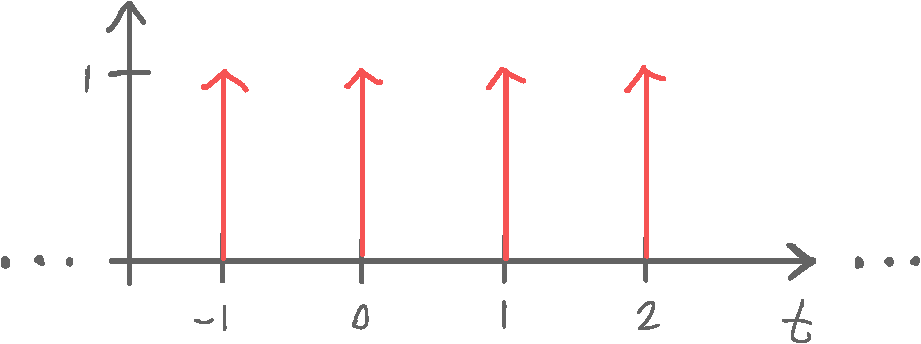
\includegraphics[width=\textwidth]{../figures/lecture01/sampling-function.pdf}
    \caption{The sampling function \eqref{eq:sampling function}, which is a mainstay of barber shops and personal care routines world-wide.}
    \label{fig:sampling function}
\end{figure}

\figref{fig:sampling function} illustrates the sampling function from \eqref{eq:sampling function}. The sampling function is also called a ``comb''\footnote{\href{https://en.wikipedia.org/wiki/Dirac_comb}{https://en.wikipedia.org/wiki/Dirac\_comb}} (you can probably guess why\dots) or an ``impulse train''.

\begin{figure}
    \centering
    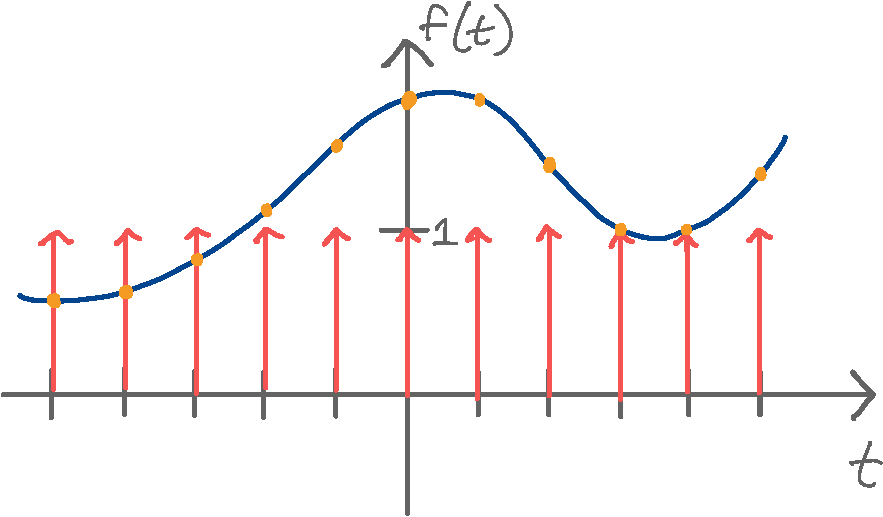
\includegraphics[width=\textwidth]{../figures/lecture01/sampling-an-arbitrary-function.pdf}
    \caption{Sampling an arbitrary function. The function is shown in blue, and the sampling function \eqref{eq:sampling function} is shown in red. The multiplication of these two functions results in a function that is 0 everywhere except where the delta functions are; at these locations, the ``value'' (loosely speaking) is the value of the blue function at that location, indicated by the orange dots.}
    \label{fig:sampling an arbitrary function}
\end{figure}

To sample an arbitrary function, we multiply it by the sampling function \eqref{eq:sampling function}, as illustrated in \figref{fig:sampling an arbitrary function}. The result is a train of impulses with integrals equal to the values of function at the locations of the Dirac impulses ($n\Delta$). Essentially, we are ``sampling'' the function at $t = n\Delta$, where $\Delta$ is referred to as the \emph{sampling period}.
Mathematically, the resulting ``sampled'' function is given by
\begin{align}
    f_\Delta(t) &= f(t) \cdot S_\Delta(t) \\
    &= \sum_{k=-\infty}^{+\infty} f(t) \delta(t - k\Delta).
\end{align}
If we are just interested in the values of the samples (which is nearly always the case), we need to integrate to find the values. For a particular sample, $k$, we have
\begin{align}
    f[k] &= \int_{-\infty}^{+\infty} f(t) \delta(t - k\Delta) \, dt \\
    &= \int_{-\infty}^{+\infty} f(k\Delta) \delta(t - k\Delta) \, dt \label{eq:sifting property}\\
    &= f(k\Delta) \underbrace{\int_{-\infty}^{+\infty} \delta(t - k\Delta) \, dt}_{= 1 \text{ by definition}} \\
    f[k] &= f(k\Delta)
\end{align}
where \eqref{eq:sifting property} is a result of the ``sifting property''\footnote{\href{https://en.wikipedia.org/wiki/Dirac_delta_function\#Translation}{https://en.wikipedia.org/wiki/Dirac\_delta\_function\#Translation}} (we leave the proof as an exercise for the reader).


\section{Quantization}

\begin{figure}
    \centering
    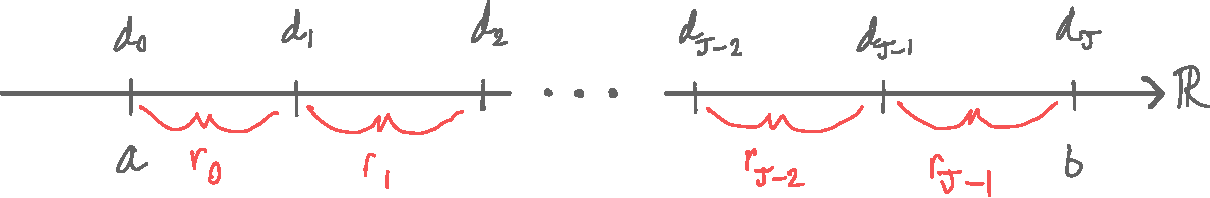
\includegraphics[width=\textwidth]{../figures/lecture01/quantization-ranges.pdf}
    \caption{Illustration of quantization. The interval $[a,b]$ is broken into sub-intervals $[d_j,d_{j+1})$; each sub-interval maps to one reconstruction level, $r_j$.}
    \label{fig:quantization ranges}
\end{figure}

Recall that quantization is a map from the real line to a finite set of values. Practically, quantization is the process of breaking a continuous range into intervals, as shown in \figref{fig:quantization ranges}. Concretely, for an interval $[a,b]$, we break the interval into $J$ ranges or ``bins'', $\left\{[d_0, d_1), [d_1, d_2),\dotsc,[d_{J-1},d_J]\right\}$; the decision of which boundary is inclusive is arbitrary, but there must be a consistent rule---$d_j$ can only belong to one interval. Each interval has an associated reconstruction value or level, $r_j$. Thus, quantization is the process of mapping any value $x \in [d_j, d_{j+1}) \mapsto r_j$.

\begin{figure}
    \centering
    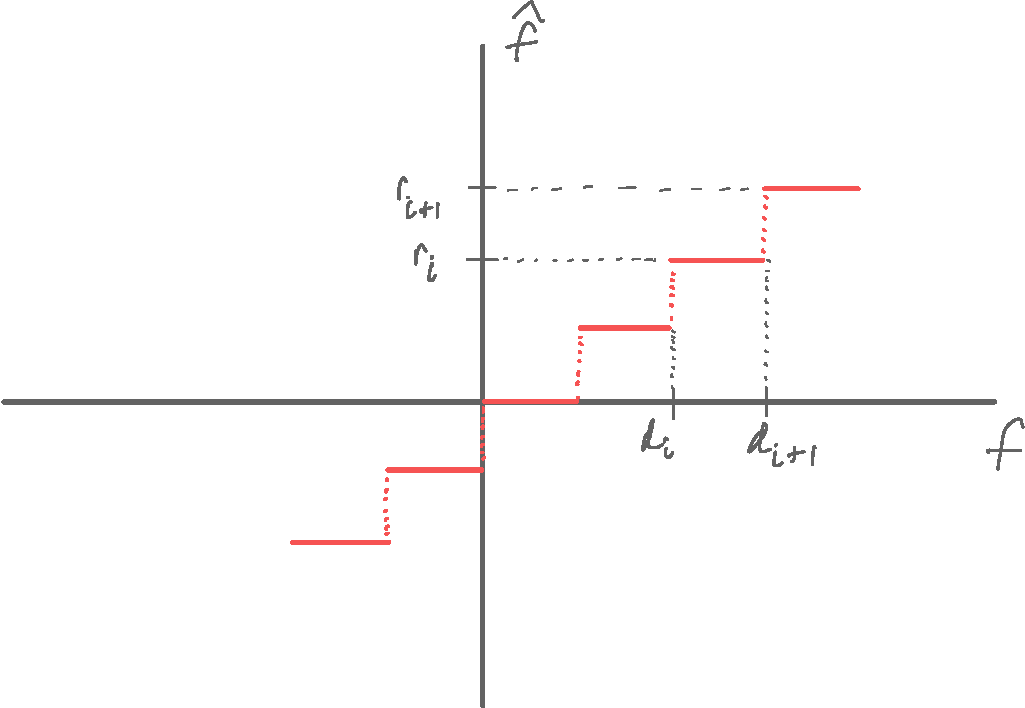
\includegraphics[width=\textwidth]{../figures/lecture01/quantization-transfer-function.pdf}
    \caption{Quantization transfer function. All values $\in [d_i, d_{i+1}) \mapsto r_i$}
    \label{fig:quantization transfer function}
\end{figure}

Quantization can also be thought of as a ``transfer function''\footnote{\href{https://en.wikipedia.org/wiki/Transfer_function}{https://en.wikipedia.org/wiki/Transfer\_function}}, $f \mapsto \hat{f}$, as shown in \figref{fig:quantization transfer function}. The transfer function is such that
\begin{equation}
    \forall \, t \in [d_j, d_{j+1}), \; \hat{f}(t) = r_j.
\end{equation}

Note that the reconstruction intervals (ranges) do not need to be uniform.

\subsection{Quantization error}
The process of mapping an entire range $[d_j,d_{j+1})$ to a single number $r_j$ represents a potentially big loss of information. Consequently, quantization leads to what is known an quantization error or quantization noise.

Assuming our signal $f$ has a probability density $p(f)$, we can calculate the mean-squared quantization error, $e$, as follows:
\begin{align}
    e &\coloneqq \mathbb{E}\left\{ (f - \hat{f}) \right\} \\
    \shortintertext{(Essentially, we are comparing the original signal to the quantized output at every value, but the comparison is weighted by the PDF)}
    &= \int_a^b (f - \hat{f})^2 p(f) \, df \\
    \shortintertext{(Since the range bins don't overlap, we can split up the integral)}
    &= \sum_{j=0}^{J-1} \int_{d_j}^{d_{j+1}} (f - r_j)^2 p(f) \, df.
\end{align}

Choosing the intervals and reconstruction levels that minimize the quantization error can be done with Llyod's algorithm\footnote{\href{https://en.wikipedia.org/wiki/Lloyd\%27s_algorithm}{https://en.wikipedia.org/wiki/Lloyd\%27s\_algorithm}} (this is the same algorithm as k-means clustering).

If we know the distribution of our signal a priori, we can choose the quantization intervals accordingly. For example, we might know that very small values and very large values are both rare, whereas values in the middle occur more commonly; thus, we could put more quantization intervals in the middle of our range, and less at the ends.

In practice, we often assume that the PDF is uniform. Under this assumption, the optimal quantization scheme (\ie, the one that minimizes the quantization error) is \emph{uniform quantization}. The uniform quantization error is given by
\begin{equation}
    \frac{(d_{j+1} - d_j)^2}{12} = \frac{\Delta^2}{12}.
\end{equation}
Under uniform quantization, the reconstruction levels, $\{r_0,\dotsc,r_{J-1}\}$, are the midpoints of their corresponding intervals.


A uniform PDF is not always a great assumption. Quantization circuits are designed and mass-produced to satisfy the needs of \emph{most} applications; consequently, manufacturers typically use uniform quantization levels.

\section{Exercises}

To gain familiarity with sampling and quantization, play around with downsampling and quantizing an audio file and listening for how the audio changes.

The following code listings show excerpts of how to do this in MATLAB. For the full listing, and implementations in other languages, visit this GitHub link:

\noindent
\href{https://github.com/johnwilliamsmithjr/BobcatTAILS/tree/main/listings/lecture01}{https://github.com/johnwilliamsmithjr/BobcatTAILS/tree/main/listings/lecture01}


\begin{listing}
    \inputminted[firstline=8, lastline=13]{Matlab}{../listings/lecture01/audiotest.m}
    \caption{Read in and play an audio file.}
    \label{lst:matlab read and play audio}
\end{listing}

\begin{listing}
    \inputminted[firstline=49, lastline=51]{Matlab}{../listings/lecture01/audiotest.m}
    \caption{Downsample the audio by a factor of 4.}
    \label{lst:matlab downsample audio}
\end{listing}

\begin{listing}
    \inputminted[firstline=68, lastline=79]{Matlab}{../listings/lecture01/audiotest.m}
    \caption{Quantize the audio.}
    \label{lst:matlab quantization}
\end{listing}





%%%%%%%%%%%%%%%%%%%%%%%%%%%%%%%%%%%%%%%%%%%%%%%%%%%%%%%%%%%%%%%%%%%%%%%%%%%%%%%%%%%%%%%%%%%%%%%%%%%%%%%%%%%%%%%%%%%%%%%%%%%%%%%%%%%%

\clearpage
\bibliographystyle{ieeetr}
\bibliography{references}

\end{document}